Zum Alphabet $\Sigma=\{\texttt{0},\texttt{1}\}$ sind die Sprachen
\[
\def\l{1}
\def\r{0.20}
\def\zustand#1{
	\draw #1 circle[radius=\r];
}
\def\akzeptierzustand#1{
	\zustand{#1}
	\draw #1 circle[radius={\r-0.05}];
}
\def\pfeil#1#2{
	\draw[->,shorten >= 0.20cm,shorten <= 0.20cm] #1 -- #2;
}
L_1
=
L\left(\raisebox{-0.85cm}{\begin{tikzpicture}[>=latex,thick]
\coordinate (q0) at (0,0);
\coordinate (q1) at (0,-1);
\clip (-0.3,-1.3) rectangle (1,0.6);
\pfeil{(0,0.8)}{(q0)}
\zustand{(q0)}
\akzeptierzustand{(q1)}
\draw[->,shorten <= 0.2cm,shorten >= 0.2cm]
	(q0) to[out=-60,in=60] (q1);
\draw[->,shorten <= 0.2cm,shorten >= 0.2cm]
	(q1) to[out=120,in=-120] (q0);
\node at ($0.5*(q0)+0.5*(q1)$) {\texttt{0}};
\draw[->,shorten <= 0.2cm,shorten >= 0.2cm]
	(q0) to[out=30,in=-30,distance=0.8cm] (q0);
\draw[->,shorten <= 0.2cm,shorten >= 0.2cm]
	(q1) to[out=30,in=-30,distance=0.8cm] (q1);
\node at ($(q0)+(0.6,0)$) [right] {\texttt{1}};
\node at ($(q1)+(0.6,0)$) [right] {\texttt{1}};
\end{tikzpicture}}
\right),\;
L_2
=
L\left(\raisebox{-0.85cm}{\begin{tikzpicture}[>=latex,thick]
\coordinate (q0) at (0,0);
\coordinate (q1) at (0,-1);
\clip (-0.3,-1.3) rectangle (1,0.6);
\akzeptierzustand{(0,0)}
\zustand{(q1)}
\pfeil{(0,0.8)}{(q0)}
\pfeil{(q0)}{(q1)}
\node at ($0.5*(q0)+0.5*(q1)$) [right] {\texttt{0},\texttt{1}};
\draw[->,shorten <= 0.2cm,shorten >= 0.2cm]
	(q1) to[out=30,in=-30,distance=0.8cm] (q1);
\node at ($(q1)+(0.6,0)$) [right] {\texttt{1}};
\end{tikzpicture}}
\right),\;
L_3
=
%\emptyset
%=
L\left(\raisebox{-0.5cm}{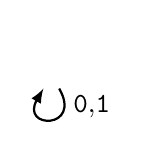
\begin{tikzpicture}[>=latex,thick]
\clip (-0.3,-0.6) rectangle (0.8,0.6);
\pfeil{(0,1)}{(0,0)}
\zustand{(0,0)}
\draw[->,shorten <= 0.2cm,shorten >= 0.2cm]
	(0,0) to[out=-60,in=-120,distance=0.8cm] (0,0);
\node at (0.15,-0.4) [right] {\texttt{0},\texttt{1}};
\end{tikzpicture}}
\right),\;
L_4
=
%\Sigma^*
%=
L\left(\raisebox{-0.5cm}{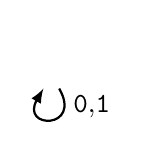
\begin{tikzpicture}[>=latex,thick]
\clip (-0.3,-0.6) rectangle (0.8,0.6);
\pfeil{(0,1)}{(0,0)}
\akzeptierzustand{(0,0)}
\draw[->,shorten <= 0.2cm,shorten >= 0.2cm]
	(0,0) to[out=-60,in=-120,distance=0.8cm] (0,0);
\node at (0.15,-0.4) [right] {\texttt{0},\texttt{1}};
\end{tikzpicture}}
\right)
\]
gegeben.
Zeichnen Sie das Zustandsdiagramm für die Sprache
$L = L_1(L_2|L_3)^*L_4$.

\themaL{regulare Ausdrucke}{reguläre Ausdrücke}

\begin{loesung}
\def\l{1.2}
\def\r{0.20}
\def\zustand#1{
	\draw #1 circle[radius=\r];
}
\def\akzeptierzustand#1#2{
	\zustand{#1}
	\draw[color=#2] #1 circle[radius={\r-0.05}];
}
\def\ehemaligerakzeptierzustand#1#2{
	\zustand{#1}
	\draw[color=#2!40,dashed] #1 circle[radius={\r-0.05}];
}
\def\pfeil#1#2{
	\draw[->,shorten >= 0.20cm,shorten <= 0.20cm] #1 -- #2;
}
Die regulären Operationen für Zustandsdiagramme ergeben
\begin{center}
\begin{tikzpicture}[>=latex,thick]
\coordinate (q0) at (0,0);
\coordinate (q1) at ({1*\l},0);
\coordinate (q2) at ({2*\l},0);
\coordinate (q3) at ({3*\l},0);
\coordinate (q4) at ({4*\l},{0.5*\l});
\coordinate (q5) at ({5*\l},{0.5*\l});
\coordinate (q6) at ({4*\l},{-0.5*\l});
\coordinate (q7) at ({2*\l},{-1*\l});
\fill[color=gray!20] ({-0.4*\l},{-0.4*\l}) rectangle ({1.4*\l},{0.9*\l});
\fill[color=gray!20] ({1.6*\l},{-1.4*\l}) rectangle ({3.1*\l},{-0.6*\l});
\fill[color=gray!20] ({3.6*\l},{0.1*\l}) rectangle ({5.9*\l},{0.9*\l});
\fill[color=gray!20] ({3.6*\l},{-0.9*\l}) rectangle ({5.1*\l},{-0.1*\l});
\pfeil{({-0.8*\l},0)}{(q0)}
\zustand{(q0)}
\draw[->,shorten <= 0.2cm,shorten >= 0.2cm]
	(q0) to[out=30,in=150] (q1);
\draw[->,shorten <= 0.2cm,shorten >= 0.2cm]
	(q1) to[out=-150,in=-30] (q0);
\node at ($0.5*(q0)+0.5*(q1)$) {\texttt{0}};
\draw[->,shorten <= 0.2cm,shorten >= 0.2cm]
	(q0) to[out=60,in=120,distance=0.8cm] (q0);
\node at ($(q0)+(0,0.5)$) [above] {\texttt{1}};
\draw[->,shorten <= 0.2cm,shorten >= 0.2cm]
	(q1) to[out=60,in=120,distance=0.8cm] (q1);
\node at ($(q1)+(0,0.5)$) [above] {\texttt{1}};
\ehemaligerakzeptierzustand{(q1)}{black}
\begin{scope}
\color{red}
\pfeil{(q1)}{(q2)}
\pfeil{(q2)}{(q3)}
\pfeil{(q3)}{(q4)}
\pfeil{(q3)}{(q6)}
\pfeil{(q2)}{(q7)}
\draw[->,shorten >= 0.2cm,shorten <= 0.2cm]
	(q4) to[out=90,in=0] ($(q4)+(-0.7,0.7)$) to[out=180,in=90] (q2);
\ehemaligerakzeptierzustand{(q2)}{red}
\zustand{(q3)}
\node at ($0.3*(q1)+0.7*(q2)$) [above] {$\varepsilon$};
\node at ($0.5*(q2)+0.5*(q3)$) [above] {$\varepsilon$};
\node at ($0.6*(q3)+0.4*(q4)$) [above] {$\varepsilon$};
\node at ($0.6*(q3)+0.4*(q6)$) [below] {$\varepsilon$};
\node at ($0.5*(q2)+0.5*(q7)$) [left] {$\varepsilon$};
\node at ($(q3)+(0,1)$) {$\varepsilon$};
\end{scope}

\ehemaligerakzeptierzustand{(q4)}{black}
\pfeil{(q4)}{(q5)}
\node at ($0.5*(q4)+0.5*(q5)+(0,-0.05)$) [above] {\texttt{0},\texttt{1}};

\zustand{(q5)}
\draw[->,shorten >= 0.2cm,shorten <= 0.2cm]
	(q5) to[out=30,in=-30,distance=0.8cm] (q5);
\node at ($(q5)+(0.5,0)$) [right] {\texttt{1}};

\zustand{(q6)}
\draw[->,shorten >= 0.2cm,shorten <= 0.2cm]
	(q6) to[out=30,in=-30,distance=0.8cm] (q6);
\node at ($(q6)+(0.5,0)$) [right] {\texttt{0},\texttt{1}};

\akzeptierzustand{(q7)}{black}
\draw[->,shorten >= 0.2cm,shorten <= 0.2cm]
	(q7) to[out=30,in=-30,distance=0.8cm] (q7);
\node at ($(q7)+(0.5,0)$) [right] {\texttt{0},\texttt{1}};
\end{tikzpicture}
\end{center}
Es ist unschwer zu erkennen, dass die akzeptierte Sprache aus Wörtern
besteht, die mindestens eine $\texttt{0}$ enthalten.
\end{loesung}
